
How do \emph{ad hoc} conventions formed through interaction with a single partner become \emph{global} conventions shared throughout a community?
Exactly how do we make the inferential leap to community-wide expectations from our experiences with specific partners? 
Grounding collective convention formation in the individual learning mechanisms explored in the previous section requires an explicit \emph{theory of generalization} capturing how people transfer what they have learned from one partner to the next.

One influential theory is that speakers simply ignore the identity of different partners and update a single monolithic representation after every interaction \cite{steels_self-organizing_1995,barr_establishing_2004,young_evolution_2015}.
We call this a \emph{complete-pooling} theory because data from each partner is collapsed into an undifferentiated pool of evidence \cite{gelman2006data}. 
Complete-pooling models have been remarkably successful at predicting collective behavior on networks, but have typically been evaluated only in settings where anonymity is enforced. 
For example, \citeA{centola_spontaneous_2015} asked how large networks of participants coordinated on conventional names for novel faces.
On each trial, participants were paired with a random neighbor but were not informed of that neighbor's identity, or the total number of different possible neighbors. 

While complete-pooling may be appropriate for some everyday social interactions, such as coordinating with anonymous drivers on the highway, it is less tenable for everyday communicative settings.
Knowledge about a partner's identity is both available and relevant for conversation \cite{eckert_three_2012, davidson_nice_1986}.
Partner-specificity thus poses clear problems for complete-pooling theories but can be easily explained by another simple model, where agents maintain separate expectations about meaning for each partner.
We call this a \emph{no-pooling} model.
The problem with no-pooling is that agents are forced to start from scratch with each partner.
Community-level expectations never get off the ground.

Our hierarchical \emph{partial-pooling} account offers a compromise between these extremes.
Unlike complete-pooling and no-pooling models, we propose that beliefs about meaning \ks{again, specific to meaning or could this also be about how meanings map to word forms or about any aspect of language?} have hierarchical structure.
That is, the meanings used by different partners are expected to be drawn from a shared community-wide distribution but are also allowed to differ from one another in systematic, partner-specific ways.
This structure provides an inductive pathway for abstract population-level expectations to be distilled from partner-specific experience.

The key predictions distinguishing our model thus concern the pattern of generalization across partners.
Experience with a single partner ought to be relatively uninformative about further partners, hence our partial-pooling account behaves much like a no-pooling model in predicting strong partner-specificity.
After interacting with enough partners in a tight-knit community, however, speakers should become increasingly confident that labels are not simply idiosyncratic features of a particular partner's lexicon but are shared across the entire community, gradually transitioning to the behavior of a complete-pooling model.
In this section, we test this novel prediction in a networked communication game and explicitly compare our model to pure complete-pooling and no-pooling variants.

\ks{There is actually a literature on how children deal with outlier language models that might be relevant here and could also strengthen your argument that we need a model that's capable of exhibiting this kind of behaviour. You can get some refs on this stuff about learning from reliable/unreliable speakers from here: https://psyarxiv.com/ruwdk}

\subsection{Model predictions}

\begin{figure*}
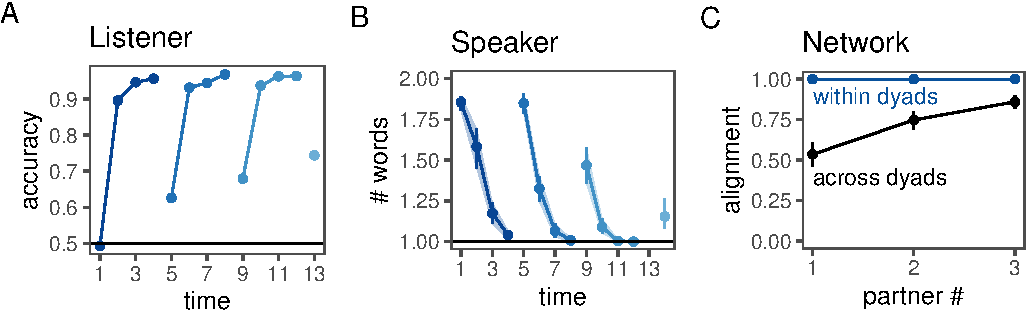
\includegraphics[scale=1.05]{./figures/sec3-model_results.pdf}
\caption{Simulation results and empirical data for (A) listener accuracy, (B) speaker reduction, and (C) network convergence across three partners. Vertical lines mark boundaries where new partners were introduced.}
\label{fig:results}
\end{figure*}

We first compare the generalization behavior produced by each model by simulating the outcomes of interacting with multiple partners on a small network. 
We used a round-robin scheme to schedule four agents into a series of repeated reference games with their three neighbors, playing 4 successive trials with one partner before advancing to the next, for a total of 12 trials.
These reference games used a set of two objects $\{o_1, o_2\}$ and four utterances $\{u_1, \dots, u_4\}$ as in Simulation 1.2, and agents swapped speaker and listener roles on each trial.
%The resulting data $D_k$ from an interaction with partner $k$ thus consisted of utterance-object pairs $\{(u, o)_t\}$ for each trial $t$, as well as information about the context of objects.

Unlike our previous simulations with a single partner, where hierarchical generalization was irrelevant, we must now specify the hyper-prior P($\Theta$) governing the overall distribution of partners (Eq.~\ref{eq:joint_inference}).
We use independent Gaussian distributions for each matrix entry $\Theta_{ij} \in \Theta$.
We then center the partner-specific prior $\phi_{ij} \in \phi$ at the corresponding value $\Theta_{ij}$:
$$\begin{array}{rcl}
P(\Theta_{ij}) & \sim & \mathcal{N}(0, 1)\\
P(\phi_{ij} | \Theta_{ij}) & \sim & \mathcal{N}(\Theta_{ij}, 1)
\end{array}$$
\ks{I just wrote "huh?" next to this in my annotated copy! :-)}
These priors represent assumptions about how far partner-specific learning can drift from the community-wide value.
We simulated 48 networks, setting $w_S = 11,~w_C = 7$ (see Fig.~\ref{fig:partnerspecificity_grid} in the Appendix for an exploration of other parameters).

%For all simulations, we used variational inference as implemented in WebPPL \cite{GoodmanStuhlmuller14_DIPPL}
%Variational methods transform probabilistic inference problems into optimization problems by approximating the true posterior with a parameterized family.
%Specifically, we make a \emph{mean-field} approximation and assume that the full posterior can be factored into independent Gaussians for each random variable. 
%We then optimize the parameters of these posterior Gaussians by minimizing the evidence lower bound (ELBO) objective \cite<see>{murphy2012machine}.
%On each trial, we run 50,000 gradient steps on previous observations to obtain a posterior (Eq.\ 1) and compute the agent's marginal prediction for the next observation by taking the expectation over 50,000 samples from the variational guide (Eq. 4)\footnote{These details were chosen to ensure high-quality estimates of the model's behavior; see Discussion for other possible algorithms.}.

\paragraph{Listener accuracy across partners}

\ks{Slightly tricky to interpret this without knowing that the community eventually converges under the pooling models - e.g. later you say ``After observing multiple partners use utterances similarly" but you haven't actually said this yet. Could consider doing convergence first, but I can see why that also works nicely last.}

We first consider the partner-specificity of a \emph{listener}'s expectations about which object is being referred to.
The probability the listener assigns to the target on each trial is shown for the different models in Fig. \ref{fig:results}A.
Under the partial-pooling model (top row), the listener agent begins at chance due to its uninformative prior, but after observing several trials of evidence from the same partner, it rapidly infers the meaning its partner is using and learns to choose the true target with higher accuracy.
When a second partner is introduced, the agent's expectations revert nearly to their original state, unlike a complete-pooling model (second row).
This reversion is due to ambiguity about whether the behavior of the first partner was idiosyncratic or attributable to community-level conventions.
In the absence of data from other partners, its observations are more parsimoniously explained at the partner-specific level.
After observing multiple partners use utterances similarly, however, we find that this knowledge has gradually been incorporated into community-level expectations. 
This is evident in much stronger initial expectations when introduced to the fourth partner ($\sim$ 75\% accuracy vs. 50\% with the first partner), unlike a no-pooling model (third row).

\paragraph{Speaker utterance length across partners}

Next, we examined our model's predictions about how a \emph{speaker}'s referring expressions will change with successive listeners.
While it has been frequently observed that messages reduce in length across repetitions with a single partner \cite{krauss_changes_1964} and sharply revert back to longer utterances when a new partner is introduced \cite{wilkes-gibbs_coordinating_1992}, the key prediction distinguishing our model concerns behavior across subsequent partner boundaries.
Complete-pooling accounts predict no reversion in number of words when a new partner is introduced  (Fig. \ref{fig:results}B, second row).
No-pooling accounts predict that roughly the same initial description length will re-occur with every subsequent interlocutor  (Fig. \ref{fig:results}B, third row). 
Here we show that a partial pooling account predicts a more complex pattern of generalization.

%As in Simulation 1.2, we allowed a set of four primitive utterances, $\{u_1, u_2, u_3, u_4\}$, to be combined into conjunctions, e.g. $\{u_1u_2, u_3u_4, \dots\}$, which are assumed to have twice the utterance cost.
%The meanings of these conjunctions were determined compositionally from the values of the primitive utterances using a standard product T-norm for conjunction. 
%Again, we introduced a weakly biased prior for $\Theta$: two of the primitive utterances were expected to apply slightly more strongly to $o_1$ and the other two more strongly to $o_2$.
%Because our values come from a Gaussian prior and the T-norm is defined over $[0,1]$, we used logistic and logit function to map values to the unit interval and back.
%Speakers do not typically begin at chance over their \emph{entire} vocabulary,
%This weak bias leads to a preference for conjunctions at the outset and thus allows us examine reduction.

First, as in Simulation 1.2, we found that descriptions become more efficient over interaction with a single partner: the model becomes more confident that shorter utterances will be meaningful, so the marginal informativity provided by the longer utterance is not worth the additional cost.
Second, we find that the speaker model reverts back to a longer description at the first partner swap: evidence from one partner is relatively uninformative about the community.
Third, after interacting with several partners, the model becomes more confident that one of the short labels is shared across the entire community, and is correspondingly more likely to begin a new interaction with it (Fig. \ref{fig:results}B, top row).

\paragraph{Network convergence}

Finally, because all agents are simultaneously making inferences about the others, the network as a whole faces a coordination problem.
For example, in the first block, agents 1 and 2 may coordinate on using $u_1$ to refer to $o_1$ while agent 3 and 4 coordinate on using $u_2$. 
Once they swap partners, they must negotiate this potential mismatch in usage. 
How does the network as a whole manage to coordinate?

We measured alignment by examining the utterances produced by speakers: if two agents produced the same utterance, we assign a 1, otherwise we assign a 0.
We compared alignment between currently interacting agents (i.e. \emph{within} a dyad) to those who were not interacting (i.e. \emph{across} dyads).
Alignment across dyads was initially near chance, reflecting the arbitrariness of whether speakers reduce to $u_1$ or $u_2$. 
Under a no-pooling model (Fig. \ref{fig:results}C, third row), subsequent blocks remain at chance, as conventions need to be re-negotiated from scratch.
Under a complete-pooling model (Fig. \ref{fig:results}C, second row), agents persist with mis-calibrated expectations learned from previous partners rather than adapting to their new partner, and \emph{within-dyad} alignment deteriorates.
By contrast, under our partial-pooling model, alignment across dyads increases without affecting alignment within dyads, suggesting that hierarchical inference leads to emergent consensus (Fig. \ref{fig:results}C, top row).

\subsection{Behavioral experiment}

\begin{figure*}
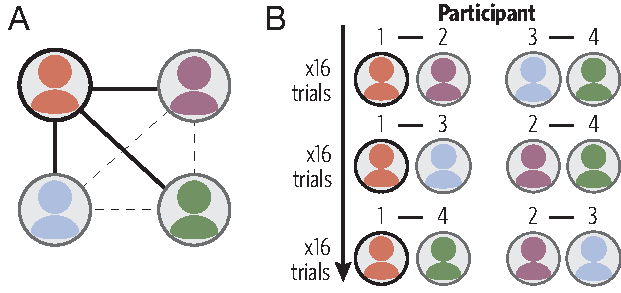
\includegraphics[scale=.95]{./figures/sec3-design.pdf}
\caption{In our experiment, (A) participants were placed in fully-connected networks of 4, (B) paired in a round-robin schedule  with each neighbor, and (C) played a series of repeated reference games using tangram stimuli.}
\label{fig:task1_display}
\end{figure*}

To evaluate the predictions observed in our simulations, we designed a natural-language communication experiment following roughly the same network design as our simulations.
That is, instead of anonymizing partners, as in many previous empirical studies of convention formation \cite<e.g.>{centola_spontaneous_2015}, we divided the experiment into blocks of extended dyadic interactions with stable, identifiable partners \cite<see>[for similar designs]{fay_interactive_2010, garrod_conversation_1994}.
Each block was a full repeated reference game, where participants had to coordinate on \emph{ad hoc} conventions for how to refer to novel objects with their partner \cite{BrennanClark96_ConceptualPactsConversation}.
Our partial-pooling model predicted that these conventions will partially reset at partner boundaries, but agents should be increasingly willing to transfer expectations from one partner to another.

\paragraph{Participants}

We recruited 92 participants from Amazon Mechanical Turk to play a series of interactive, natural-language reference games. 
%Base pay was set to \$3.00, with a 4 cent performance bonus for each correct response.

\paragraph{Stimuli and procedure}

Each participant was randomly assigned to one of 23 fully-connected networks with three other participants as their 'neighbors' (Fig. \ref{fig:task1_display}A). 
Each network was then randomly assigned one of three distinct "contexts" containing abstract tangram stimuli taken from \cite{ClarkWilkesGibbs86_ReferringCollaborative}.
The experiment was structured into a series of three repeated reference games with different partners, using these same four stimuli as referents.
Partner pairings were determined by a round-robin schedule (Fig. \ref{fig:task1_display}B).
The trial sequence for each reference game was composed of four repetition blocks, where each target appeared once per block.
Participants were randomly assigned to speaker and listener roles and swapped roles on each block.
After completing sixteen trials with one partner, participants were introduced to their next partner and asked to play the game again. 
This process repeated until each participant had partnered with all three neighbors.
Because some pairs within the network took longer than others, we sent participants to a temporary waiting room if their next partner was not ready. 

Each trial proceeded as follows.
First, one of the four tangrams in the context was highlighted as the \emph{target object} for the speaker.
They were instructed to use a chatbox to communicate the identity of this object to their partner, the listener (see Fig. \ref{fig:task1_display}C).
The two participants could engage freely in dialogue through the chatbox but the listener must ultimately make a selection from the array. 
Finally, both participants in a pair were given full feedback on each trial about their partner's choice and received bonus payment for each correct response. 
The order of the stimuli on the screen was randomized on every trial to prevent the use of spatial cues (e.g. 'the one on the left').
The display also contained an avatar representing their current partner to emphasize that they were speaking to the same partner for an extended period. \ks{Are the distinct avatars as shown in Fig 8C? It looks relatively subtle there, just different shades?}

\subsection{Results}


We evaluated participants' generalization behavior on the same three metrics we used in our simulations: accuracy, utterance length, and network convergence.

\paragraph{Listener accuracy}

We first examined changes in the proportion of correct listener selections.
In particular, our partial pooling model predicts (1) gains in accuracy within each partner and (2) drops in accuracy at partner boundaries, but (3) overall improvement in initial interactions with successive partners.
To test the first prediction, we constructed a logistic mixed-effects regression predicting trial-level listener responses. 
We included a fixed effect of repetition block within partner (1, 2, 3, 4), along with random intercepts and slopes for each participant and each tangram. 
We found that accuracy improved over successive repetitions with every partner, $b=0.69,z=3.87, p<0.001$.

To test changes at partner boundaries, we constructed another regression model.
We coded the repetition blocks immediately before and after each partner swap, and included this as a categorical fixed effect.
Because partner roles were randomized for each game, the same participant often did not serve as listener in both blocks, so in addition to tangram-level intercepts, we included random slopes and intercepts at the \emph{network} level (instead of the participant level).
We found that across the two partner swaps, accuracy dropped significantly, $b = -1.56, z = -2, p < 0.05$\ks{give exact p, even if it's pretty much bang on .05}, reflecting partner-specificity of meaning \ks{"reflecting partner-specificity of meaning" - somehow this wording confused me, is it clearer to say that it reflects the fact that the population has not completely converged on a shared system of meaning / meaning-form mapping?}.
Finally, to test whether performance improves for the \emph{very first} interaction with each new partner, before observing any partner-specific information, we examined the simple effect of partner number on the trials immediately after the partner swap ($t=\{1,5,9\}$).
As predicted, we found a significant improvement in performance, $b = 0.57, z = 2.72, p < 0.01$, suggesting that listeners are bringing increasingly well-calibrated expectations into interactions with novel neighbors (see Fig. \ref{fig:results}A, bottom row).

%\begin{figure*}
%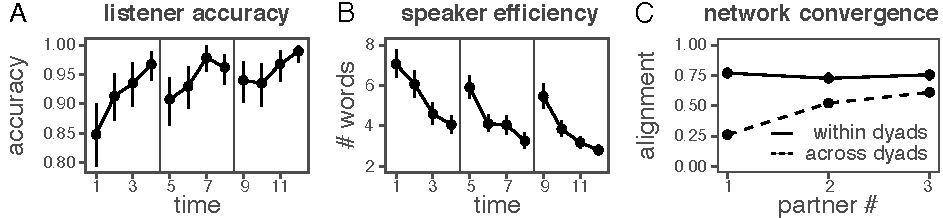
\includegraphics[scale=1.1]{./figures/sec3-empirical-results.pdf}
%\caption{Results from networked communication experiment. (A) Increase in accuracy across partners, (B) reduction in number of words across partners, (C) network convergence.}
%\label{fig:results}
%\end{figure*}


\paragraph{Speaker utterance length}

Next, as a measure of coding efficiency, we calculated the raw length (in words) of the utterance produced on each trial.
We then tested analogues of the same three predictions we tested in the previous section using the same mixed-effects models, but using a linear regression on the continuous measure of efficiency instead of accuracy (see Fig. \ref{fig:results}B, bottom row).
We log-transformed utterance lengths for stability \ks{stability in what sense?}.
We found that speakers reduced utterance length with every partner, $b = -0.19, t(34) = -9.88, p < 0.001$, increased length across partner-boundaries, $b = 0.43, t(22) = 4.4, p < 0.001$, and decreased the length of their \emph{initial descriptions} with each new partner on their network,, $b = -0.2, t(516.5) = -6.07, p < 0.001$ (see Fig. \ref{fig:results}B, bottom row).

\paragraph{Network convergence }

In this section, we examine the actual \emph{content} of pacts and test whether these coarse signatures of generalization actually lead to increased alignment across the network, as predicted. 
Specifically, we extend the `exact matching' measure of alignment used in Simulation 3 to natural language production by examining whether the \emph{intersection} of words produced by different speakers was non-empty.
We excluded a list of common stop words (e.g. 'the', 'both') to focus on the core conceptual content of pacts; using a continuous measure based on the size of the intersection instead of a binary measure yielded similar results.

As in our simulation, the main comparison of interest was between currently interacting participants and participants who are not interacting: we predicted that within-pair alignment should stay consistently high while (tacit) alignment between non-interacting pairs will increase. 
We thus constructed a mixed-effects logistic regression including fixed effects of pair type (within vs. across), partner number, and their interaction.
We included random intercepts at the tangram level and maximal random effects at the network level (i.e. intercept, both main effects, and the interaction).
As predicted, we found a significant interaction ($b = -0.85, z = -5.69, p < 0.001$; see Fig. \ref{fig:results}C, bottom row).
Although different pairs in a network may initially use different labels, these labels begin to align over subsequent interactions. 

\subsection{Discussion}

Our partial pooling model claims\ks{assumes?} that conventions represent the shared structure that agents "abstract away" from partner-specific learning.
In this section, we evaluated the extent to which our partial pooling model captured human generalization behavior in a natural-language communication experiment on small networks.
Unlike complete-pooling accounts, our model allows for partner-specific common ground to override community-wide expectations given sufficient experience with a partner, or in the absence of strong conventions.
Unlike no-pooling accounts, it allows\ks{results in?} networks to converge on more efficient and accurate expectations about novel partners.

While it is not easily classified into either the complete-pooling or no-pooling classes, the priming mechanisms proposed by \emph{interactive alignment} accounts also cannot straightforwardly account for patterns of partner-specificity.
If a particular semantic representation has been activated due to precedent in the preceding dialogue, then the identity of the speaker should not in principle alter its continued influence \cite{brennan2009partner}.
More sophisticated hierarchical memory retrieval accounts that represent different partners as different \emph{contexts} \cite<e.g>{polyn2009context} may be consistent with partner-specificity, but evoking such an account presupposes that social information like partner identity is already a salient and relevant feature of the agent's context representation and thus no longer relies purely on ``egocentric'' priming and activation mechanisms. \ks{I know you guys are not big fans of priming, but is it fairer to say that they need to be augmented with social info to capture this kind of result, rather than saying they "cannot" at the start here? I think there's a bunch of converging evidence that that's the case.}
Indeed, a process-level account assuming socially-aware context reinstatement for episodic memories, and slower consolidation of shared features into population-level expectations, may be one possible candidate for realizing our computational-level model (see General Discussion for more on process-level evidence).

%A frequent concern in prior work using repeated reference games is that improvements in communication over time are due to generic effects of task familiarity and repetition rather than interactive adaptation to a partner's language use \cite{HupetChantraine92_CollaborationOrRepitition}.
%As they get more practice with the task, speakers may simply get better overall at describing images and listeners may learn how to better identify target images. 
%The effects we observe at partner boundaries show that something is being learned beyond pure familiarity with the task: if speakers and listeners were just learning to better describe and identify targets regardless of who their partner is, we would not expect these reversions.
%These partner-specificity effects clearly rule out the complete pooling model with a practice effect confound, but cannot rule out a no-pooling model with a practice effect confound.
%Under this null hypothesis, partner-specific adaptation would be genuine, but the general decrease in utterance length and increase in accuracy with new partners would due to practice rather than inductive generalization.

%Our best evidence against this null model lies in our network convergence results: networks as a whole converge to similar short descriptions across partners, and different networks converge to different descriptions.
%This finding is inconsistent with a pure practice effect: each speaker and listener would be expected to each individually get better at efficient description and accurate identification across partners, but not to tailor those efficient descriptions to the apparent and emerging conventions of their network.
%Future work may also address these concerns by testing generalization across different stimuli sets (with the same partner), rather than across different partners (with the same stimuli). 
%Our account predicts that similar inductive learning mechanisms would operating over the stimulus axis as the partner axis: partial reversions to the prior would be expected at stimulus set boundaries, given the stimulus-specificity of pacts, but then participants would be expected to gradually abstract away common structure (e.g. the dimensional structure of the stimulus space) that can be expected to transfer to new stimuli with the same partner. 
%Critically, if then switched to a new partner after an equivalent number of trials, we should still see significant reversion along the partner-specificity axis.
%This would be a stronger test of evidence against pure practice effects. 


%While our behavioral data appears inconsistent with complete-pooling and no-pooling accounts, there remain deep theoretical connections between our hierarchical Bayesian formulation and alternative theories of generalization which may also be considered ``partial-pooling'' \cite{rogers2004semantic,marcus2018algebraic,doumas2008theory}.
%For example, recent neural network algorithms such as Model-Agnostic Meta-Learning \cite<MAML>{FinnAbeelLevine17_MAML}, which attempt to learn general parameter settings (e.g. conventions) that can rapidly adapt to different specific tasks (e.g. partners), have been shown to be equivalent to hierarchical Bayes under certain conditions \cite{grant_recasting_2018}.
%Such neural network instantiations may scale better in practice to natural language in more complex referential spaces, and may only require a handful of gradient steps to successfully adapt \cite{hawkins2019continual}.
%Alternatively, if different partners are represented as different contexts \cite{brown2015people}, then appropriately hierarchical reinforcement learning mechanisms may produce similar predictions \cite{gershman2015novelty}.
%These theoretical connections expose a common underlying view that conventions emerge from a group of agents discovering latent structure in coordination problems by adapting to each idiosyncratic partner along the way.
